\documentclass[sigconf]{acmart}
\usepackage{lmodern}
\usepackage[T1]{fontenc}
\usepackage{graphicx}
\usepackage{amsmath}
\usepackage{booktabs}
\usepackage{float}
\usepackage{placeins}
\begin{document}
	\title{Analysis and Evaluation of Machine Learning Operations on a Show Recommendation System}
	\author{Marco De Rito
		Data Engineer}
	\affiliation{%
		\institution{Università degli Studi di Trieste}
		\streetaddress{Piazzale Europa, 1, 34127}
		\city{Trieste}
		\country{Italy}}
	\email{marco.derito@studenti.units.it}
	\begin{abstract}
		In this paper, I present the development and evaluation of a recommendation system for a streaming platform. The primary goal was to create personalized user profiles and to segment the catalogue of shows into distinct clusters based on user preferences using machine learning techniques. The project employed K-Means clustering for segmentation and a Random Forest classifier for recommendation. The results demonstrated a high accuracy of 82\%, with various evaluation metrics indicating the robustness of the model.
	\end{abstract}
	\keywords{Recommendation System; Machine Learning; Streaming Platform; User Profiles; Clustering; K-Means; Random Forest; TF-IDF; Data Preprocessing; Silhouette Score; Confusion Matrix; ROC Curve; AUC; Precision-Recall Curve; Feature Importance; Bootstrap Sampling; Ensemble Methods; Computational Resources Optimization; Deep Learning; Filter Bubble; Dimensionality Reduction; Unstructured Data; User Reviews.}
	\maketitle
	\section{Introduction}
	In the digital age, the vast amount of content available on streaming platforms has created a paradox of choice for users. With thousands of movies, TV shows, and documentaries available at their fingertips, users often struggle to find content that aligns with their preferences. Recommendation systems have emerged as a crucial tool in addressing this challenge, providing personalized suggestions based on user behavior and preferences. This project aims to develop a recommendation system for a streaming platform using machine learning techniques. The primary objective was to create personalized user profiles based on their viewing habits and preferences and to segment the catalogue of shows into distinct clusters. By implementing this system, the platform can deliver content that is highly relevant to each user, thereby enhancing user satisfaction and reducing the time spent searching for content.
	\section{Background}
	Datasets used in this project were sourced from Kaggle, a well-known platform for sharing machine learning datasets. Specifically, the "Netflix Movies and TV Shows" dataset provided by Rahul Vyas was utilized \cite{kaggle_dataset}. This dataset includes comprehensive information on a variety of shows available on a streaming platform, such as titles, genres, directors, cast, countries of origin, ratings, and user reviews. These data points are vital for constructing user profiles and for the machine learning algorithms to make accurate predictions and recommendations.
	
	Additionally, to enrich the dataset with user ratings, we performed an \texttt{INNER JOIN} operation between this original dataset and the "Netflix Movie Rating" dataset provided by Rishit Javia on Kaggle \cite{netflix_ratings}. This join operation allowed us to combine the show metadata with user ratings, creating a more comprehensive dataset for the recommendation system.
	
	Furthermore, additional ratings were collected from a small group of participants within our personal network. These ratings were integrated into the dataset to supplement the existing data and to test the recommendation system's ability to handle new, real-world data.
	
	The primary techniques employed in this project include clustering for segmentation and a Random Forest classifier for recommendation. Clustering was used to group similar shows, creating distinct profiles that reflect various user tastes. The Random Forest model, known for its robustness and effectiveness in handling complex datasets, was then used to classify and recommend content based on these profiles.
	\section{Methodology/Approach}
	\subsection{Data Preprocessing}
	Data preprocessing is a critical step in any machine learning project, as it ensures the quality and consistency of the input data. In this project, preprocessing involved several key steps:
	\begin{itemize}
		\item \textbf{Handling Missing Data}: Any missing values in the dataset were either filled in or the corresponding entries were removed to ensure data integrity.
		\item \textbf{Textual Data Transformation}: Textual variables such as titles, genres, and cast names were converted into numerical formats using the \texttt{TfidfVectorizer}. This vectorization process involves calculating the Term Frequency-Inverse Document Frequency (TF-IDF) for each term in the text data, which measures how important a word is to a document in a collection. The TF-IDF value is computed as follows:
	\end{itemize}
	\begin{equation}
		\text{TF-IDF}(t, d) = \text{TF}(t, d) \times \text{IDF}(t)
	\end{equation}
	where:
	\begin{itemize}
		\item $\text{TF}(t, d)$ is the term frequency of term $t$ in document $d$.
		\item $\text{IDF}(t)$ is the inverse document frequency of term $t$ across all documents.
	\end{itemize}
	This method transforms the text data into a numerical matrix, which can then be used as input for machine learning algorithms.
	\subsection{Clustering Using K-Means}
	Clustering is a technique used to group similar data points into clusters. In this project, K-Means clustering was applied to segment the shows into distinct profiles. The K-Means algorithm works by partitioning the data into $k$ clusters, where each data point belongs to the cluster with the nearest mean. The process involves:
	\begin{enumerate}
		\item \textbf{Initialization}: Randomly selecting $k$ initial centroids.
		\item \textbf{Assignment Step}: Assigning each data point to the nearest centroid based on Euclidean distance.
		\item \textbf{Update Step}: Recalculating the centroids by taking the mean of all points assigned to each centroid.
		\item \textbf{Repeat}: Repeating the assignment and update steps until the centroids no longer change.
	\end{enumerate}
	The silhouette score was used to determine the optimal number of clusters ($k$). The silhouette score is a measure of how similar an object is to its own cluster compared to other clusters, and is calculated as follows:
	\begin{equation}
		\text{Silhouette Score} = \frac{b - a}{\max(a, b)}
	\end{equation}
	where:
	\begin{itemize}
		\item $a$ is the average distance between a data point and all other points in the same cluster.
		\item $b$ is the average distance between a data point and all other points in the nearest cluster.
	\end{itemize}
	A silhouette score close to 1 indicates that the data points are well-clustered.
	\subsection{Random Forest Classifier for Recommendation}
	Random Forest is an ensemble learning method that operates by constructing a multitude of decision trees during training and outputting the mode of the classes for classification. The Random Forest algorithm can be described as follows:
	\begin{enumerate}
		\item \textbf{Bootstrap Sampling}: Randomly selecting samples from the dataset with replacement to create multiple training subsets.
		\item \textbf{Decision Tree Construction}: Building decision trees on each subset. Each tree is trained on a different random subset of features.
		\item \textbf{Voting}: Aggregating the predictions from each tree to determine the final output.
	\end{enumerate}
	The Random Forest classifier is particularly well-suited for this project due to its ability to handle large datasets with numerous features and its resistance to overfitting. The classifier was trained using the training dataset, and its performance was evaluated on a separate test set using various metrics.
	\subsection{Evaluation Metrics}
	Several evaluation metrics were used to assess the performance of the model:
	\begin{itemize}
		\item \textbf{Confusion Matrix}: Summarizes the true positives, true negatives, false positives, and false negatives, providing a clear overview of classification performance.
		\item \textbf{Classification Report}: The classification report provides a detailed analysis of the model’s performance, breaking it down by precision, recall, and F1-score for each class. This report helps to identify how well the model is performing across different categories, with high precision indicating a low rate of false positives, and high recall indicating a low rate of false negatives. The F1-score, a harmonic mean of precision and recall, offers a balanced metric particularly useful when dealing with class imbalance.
		\item \textbf{ROC Curve and AUC}: The ROC curve plots the true positive rate against the false positive rate, and the Area Under the Curve (AUC) provides a single measure of the model's ability to distinguish between classes. An AUC closer to 1 indicates better performance.
		\item \textbf{Precision-Recall Curve}: Particularly useful for imbalanced datasets, this curve shows the trade-off between precision (the accuracy of positive predictions) and recall (the ability to identify all positive instances).
		\item \textbf{Feature Importance}: Analyzing the importance of different features in the Random Forest model revealed which attributes were most influential in predicting user preferences, with certain genres, release years, and durations being particularly significant.
	\end{itemize}
	\section{Visualization of Data and Results}
	\subsection{EDA}
	Several graphs were generated to visualize the data and the results:
	\begin{itemize}
		\item \textbf{Genre Distribution} (Figure 1): The genre distribution graph illustrated how genres were grouped in the dataset. This graph provided insight into which genres were more prevalent and how they contributed to the clustering process.
		\begin{figure}[H]
			\centering
			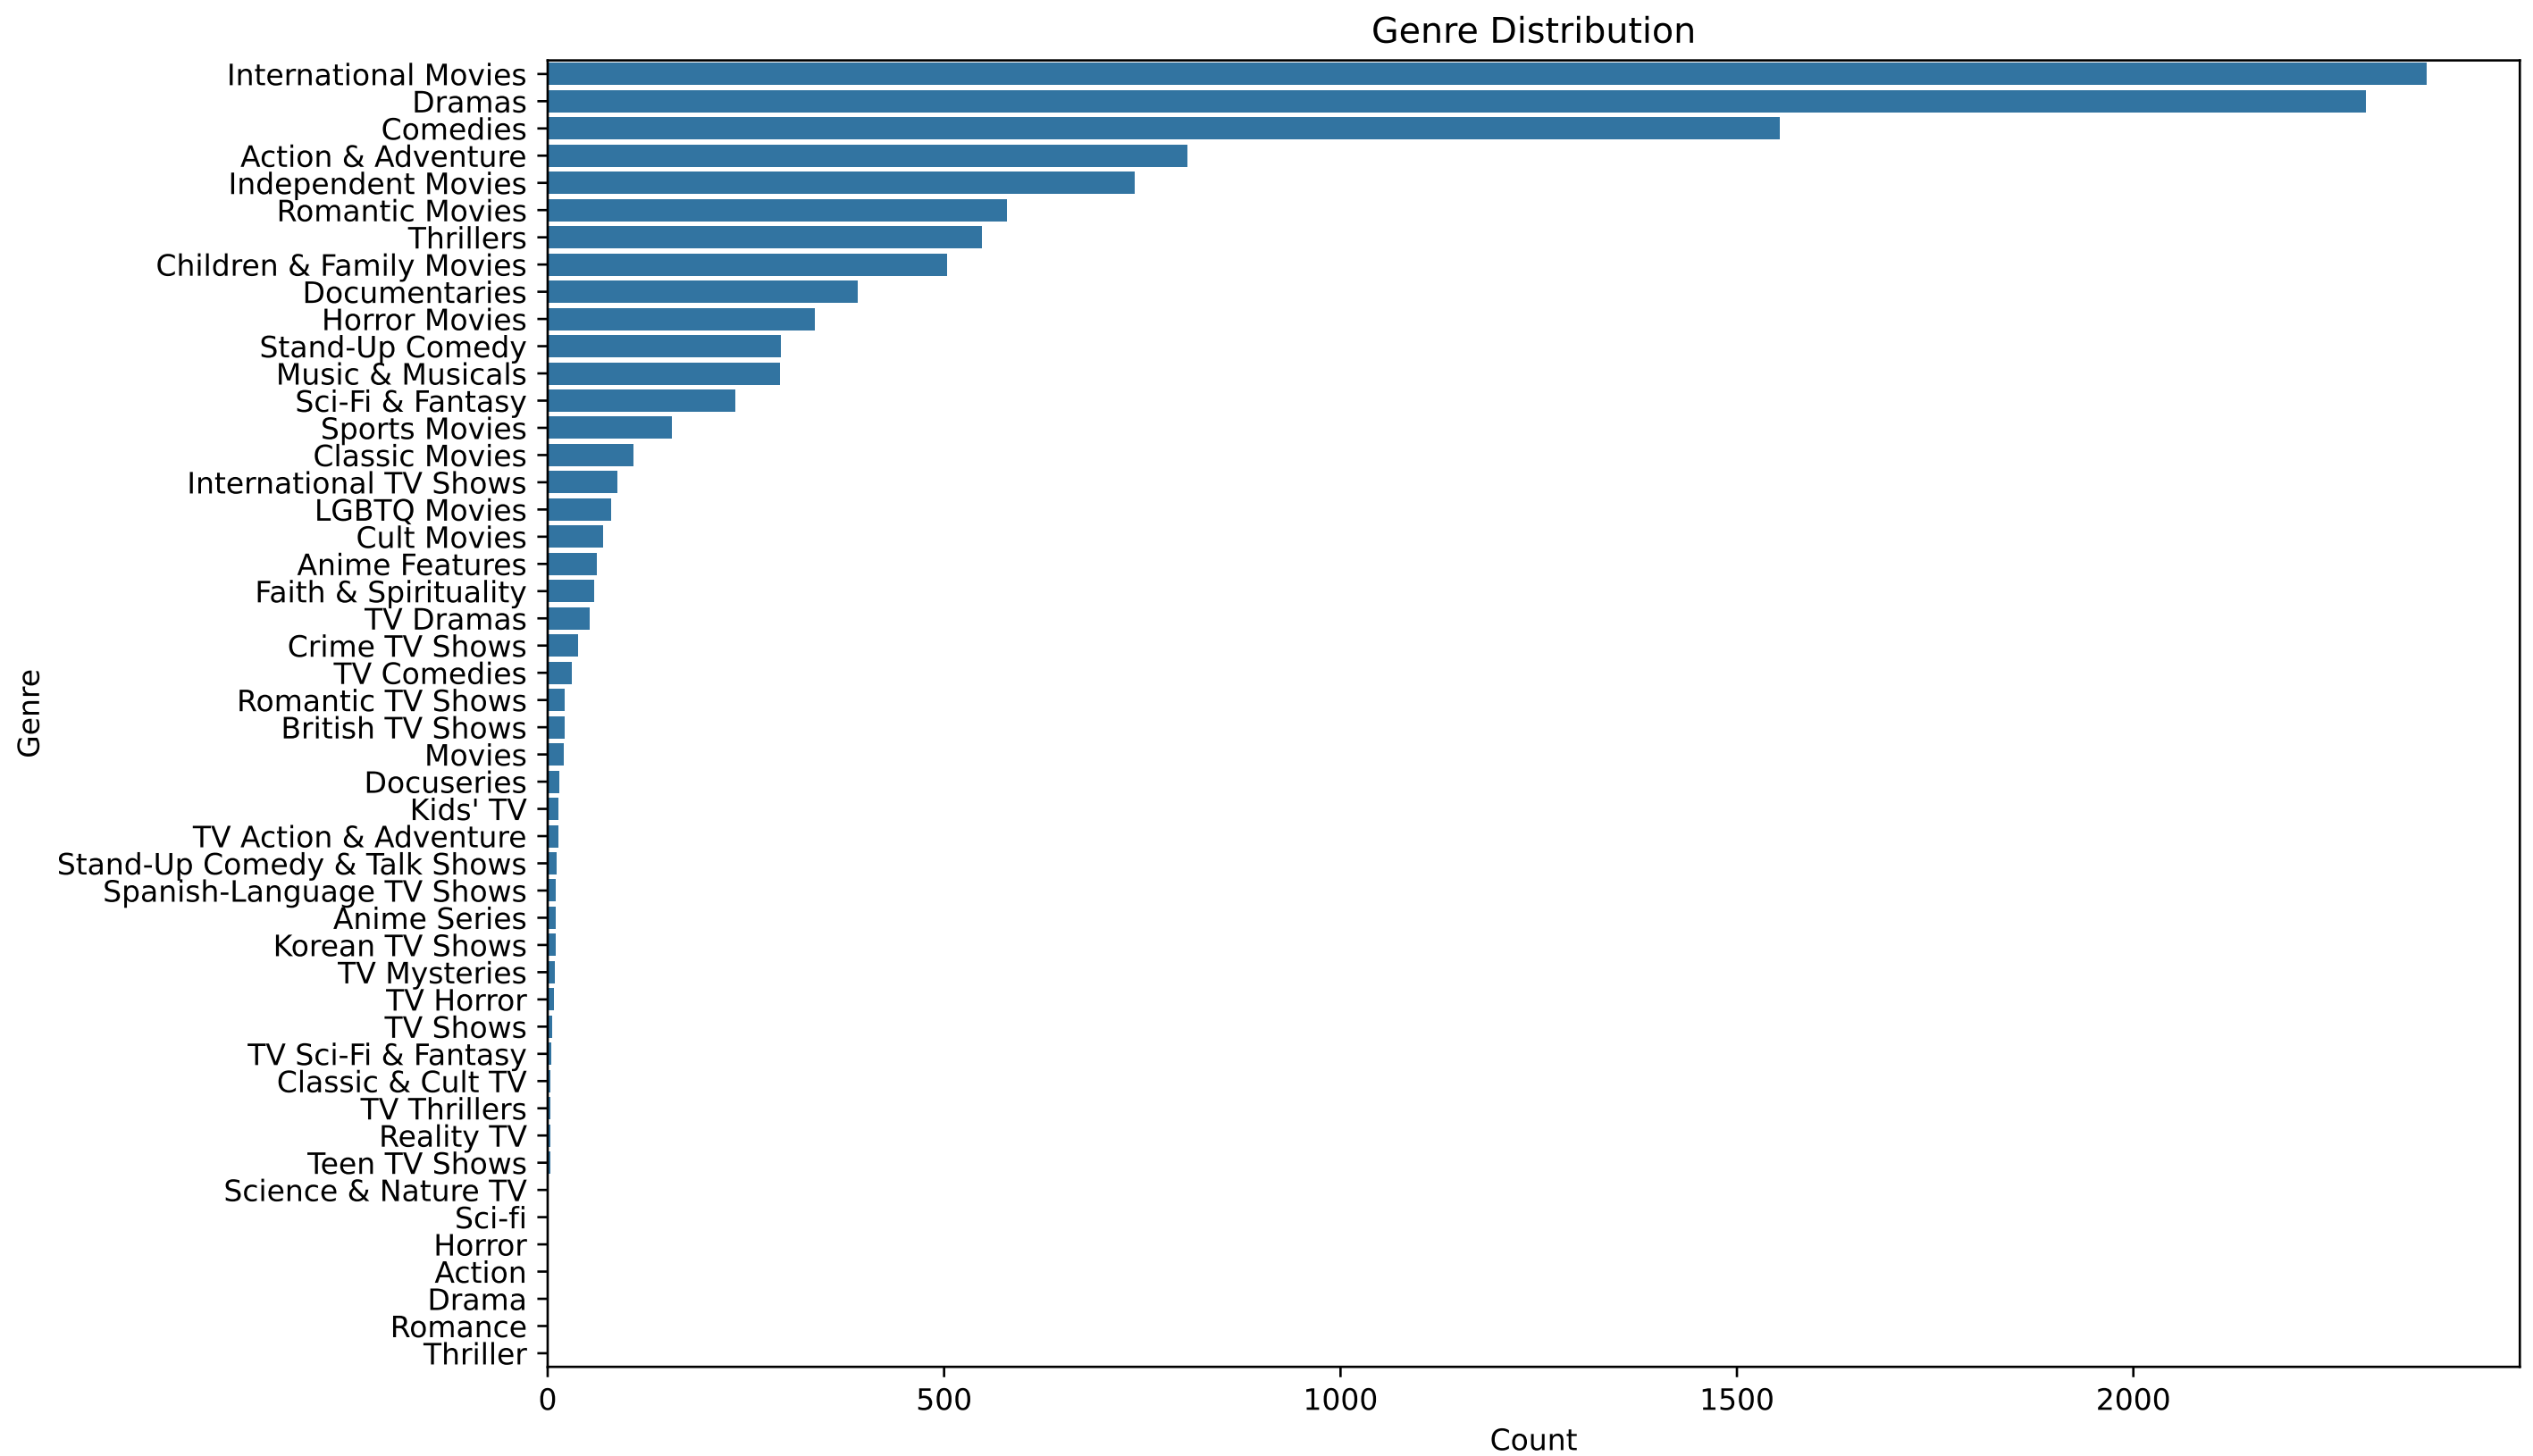
\includegraphics[width=0.5\textwidth]{C:/Users/marco/OneDrive/Documents/GitHub/mlops-netflix/mdr/plots/GenreDistribution.png}
			\caption{Genre Distribution}
			\label{fig:genre_distribution}
		\end{figure}
		\FloatBarrier
		\item \textbf{Pairplot of Numerical Variables} (Figure 2): The pairplot provided a comprehensive view of the relationships between numerical variables, such as show duration and release year. This visualization helped identify potential correlations that could be leveraged to improve the recommendation system.
		\begin{figure}[H]
			\centering
			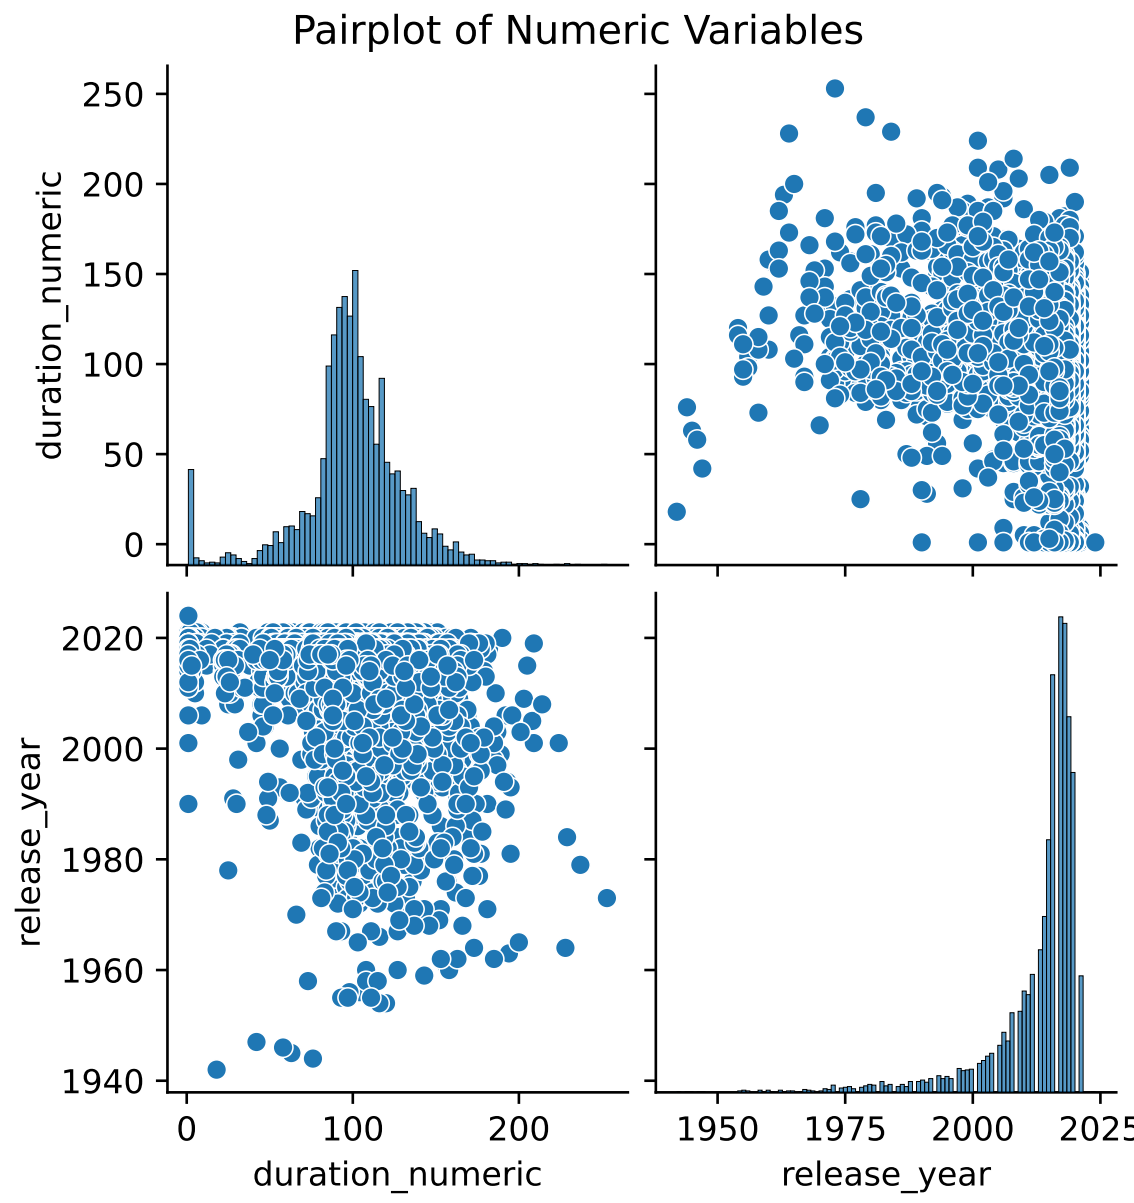
\includegraphics[width=0.5\textwidth]{C:/Users/marco/OneDrive/Documents/GitHub/mlops-netflix/mdr/plots/PairPlotNumericVariables.png}
			\caption{Pairplot of Numerical Variables}
			\label{fig:Pairplot}
		\end{figure}
		\FloatBarrier
		\item \textbf{Like/Dislike Distribution} (Figure 3): By analyzing the distribution of likes and dislikes from the \texttt{ratings.csv} file, the project was able to identify which shows were more favored by users. This analysis was crucial for refining the recommendation system to align with user preferences.
	 	\begin{figure}[H]
		\centering
		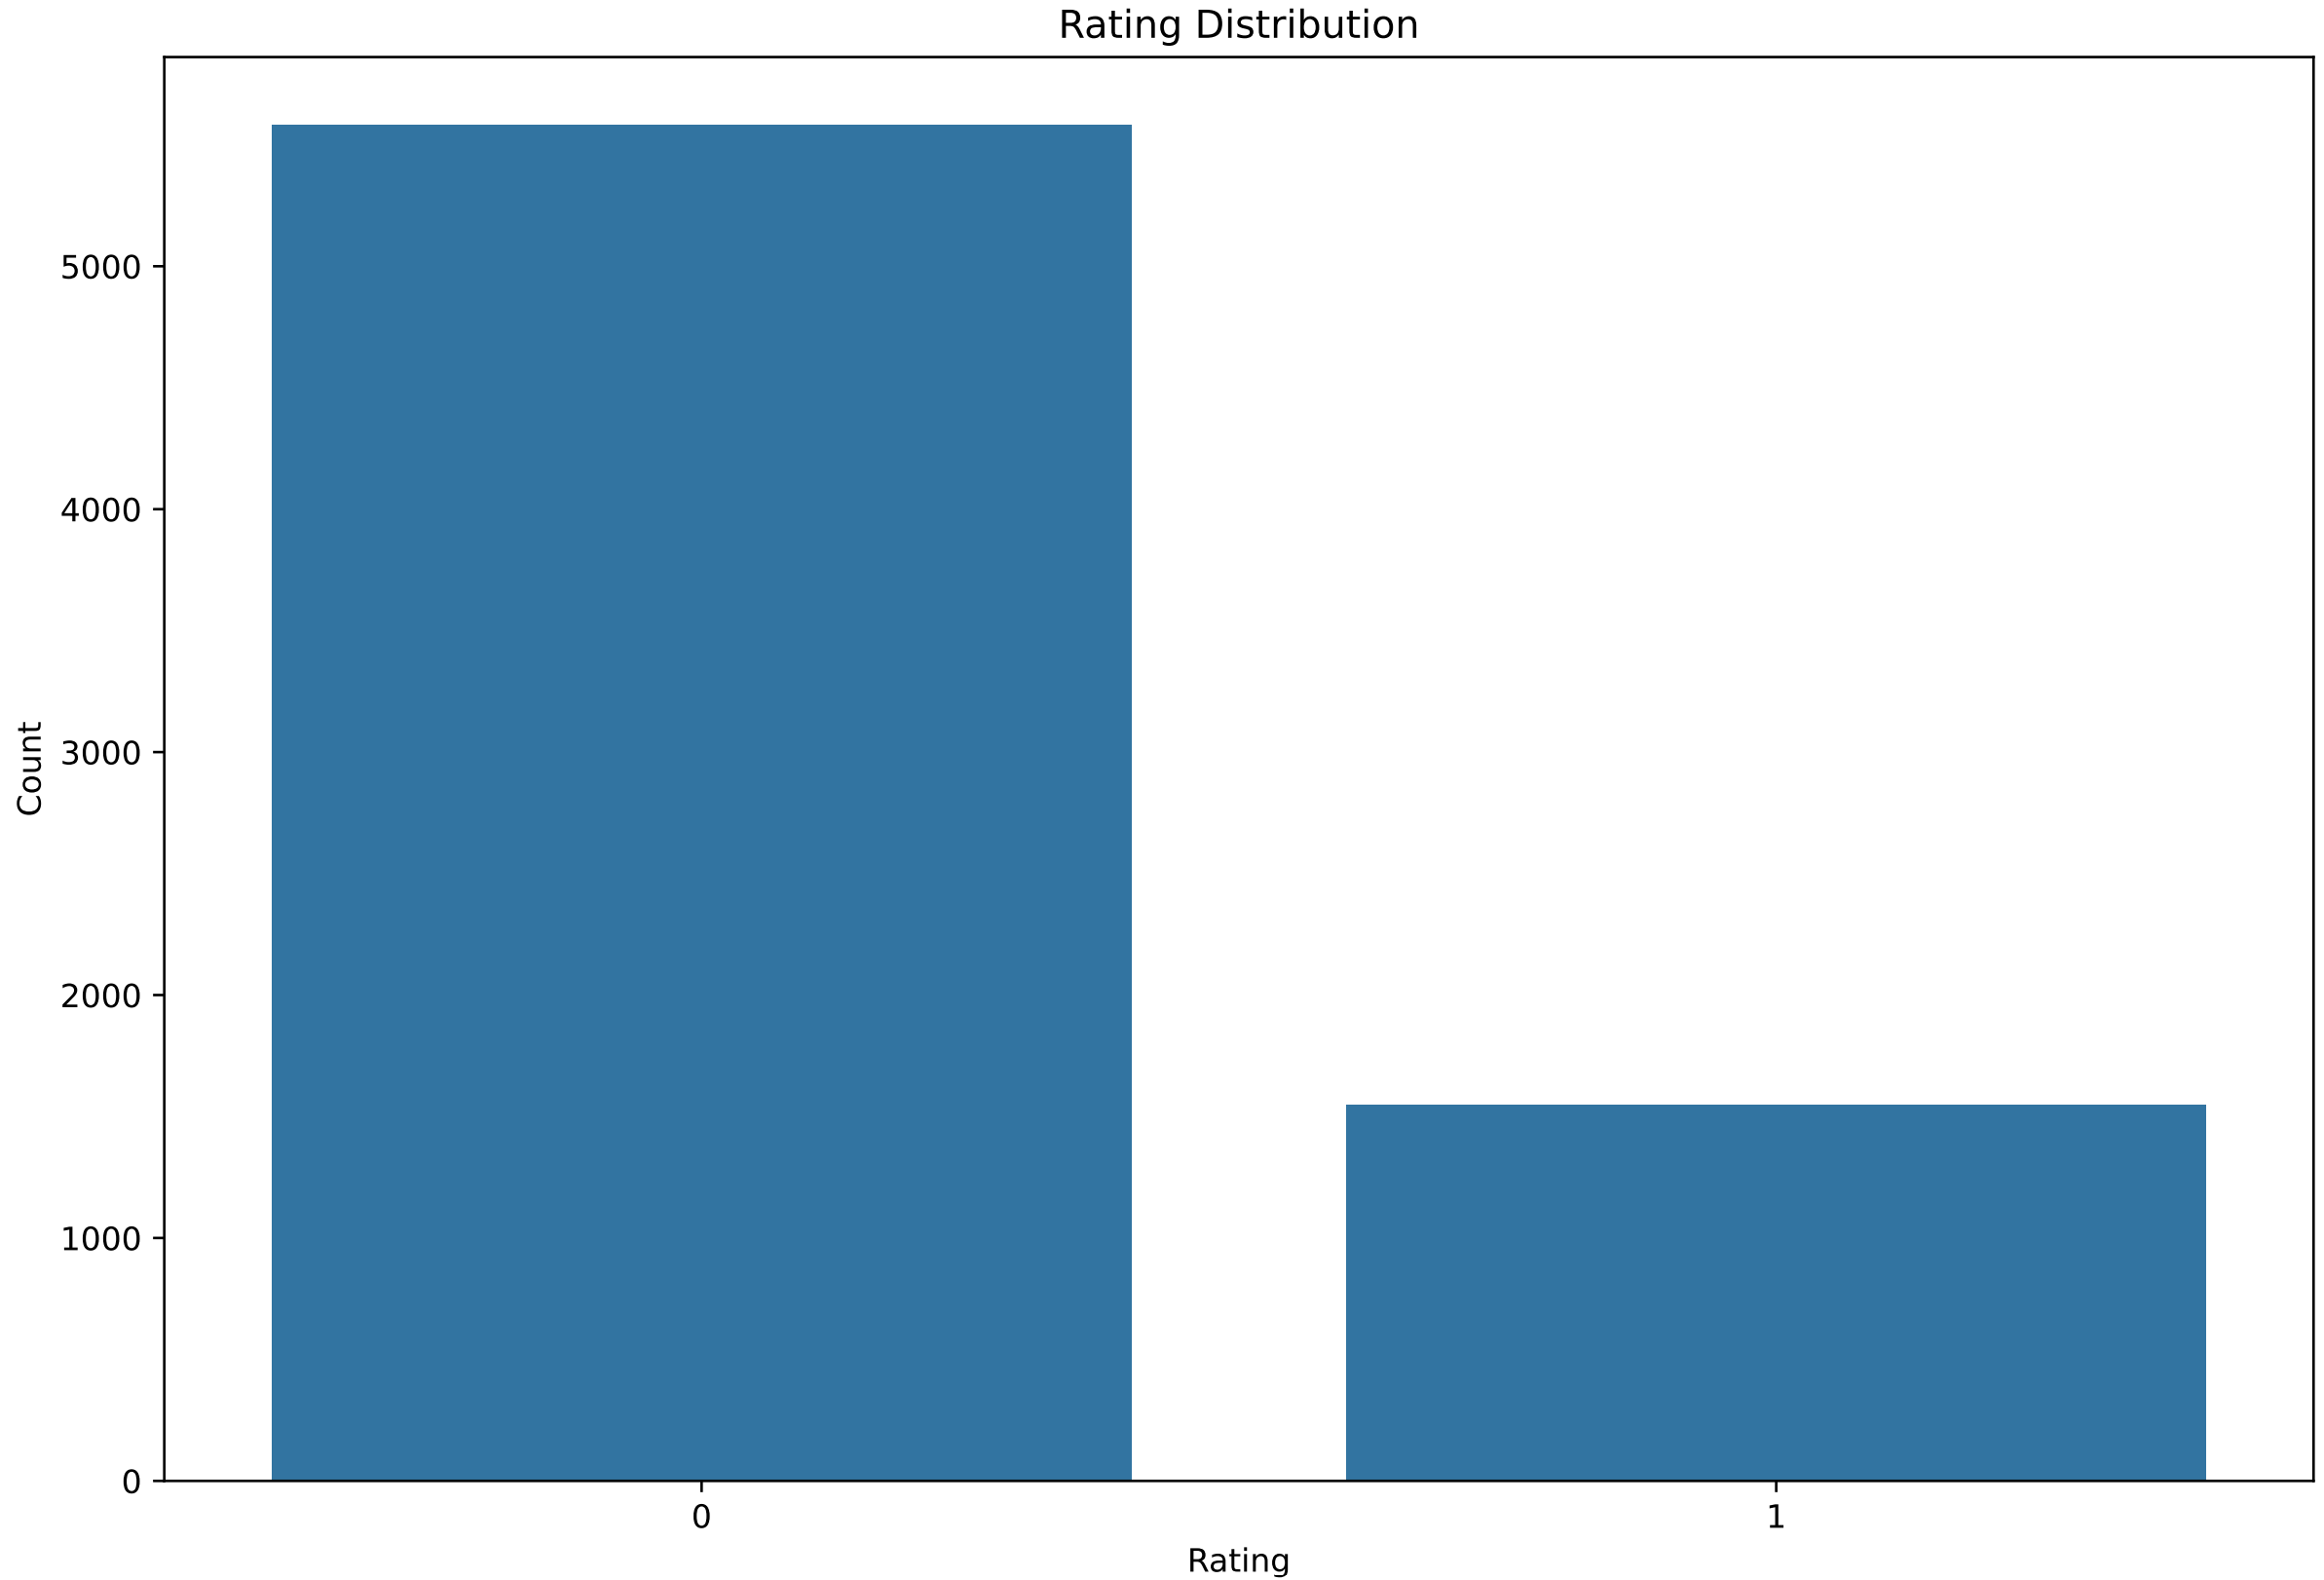
\includegraphics[width=0.5\textwidth]{C:/Users/marco/OneDrive/Documents/GitHub/mlops-netflix/mdr/plots/RatingDistribution.png}
		\caption{Like/Dislike Distribution}
		\label{fig:RatingDistribution}
		\end{figure}
		\FloatBarrier
	\end{itemize}
	\subsection{Analysis of Statistical Results}
	The Random Forest model achieved an overall accuracy of 82\%, which indicates a strong performance in classifying and recommending shows based on user profiles. To further analyze the model's performance, several key metrics were examined:
	\begin{itemize}
		\item \textbf{Classification Report} (Figure 4): The classification report offers a detailed breakdown of the model’s performance across different classes. It includes metrics such as precision, recall, and F1-score for each class. The report for this project revealed:
			\begin{itemize}
				\item \textbf{Class 0.0} - Precision: 0.89, Recall: 0.74, F1-Score: 0.81. This indicates that the model is highly precise but could improve in recalling all true positive instances.
				\item \textbf{Class 1.0} - Precision: 0.76, Recall: 0.90, F1-Score: 0.83. This shows a slightly lower precision but very high recall, meaning the model is effective at capturing almost all true positive instances for this class.
				\item \textbf{Macro and Weighted Averages} - Both averages are around 0.82 for precision, recall, and F1-score, reflecting balanced performance across classes.
			\end{itemize}
			\begin{figure}[H]
				\centering
				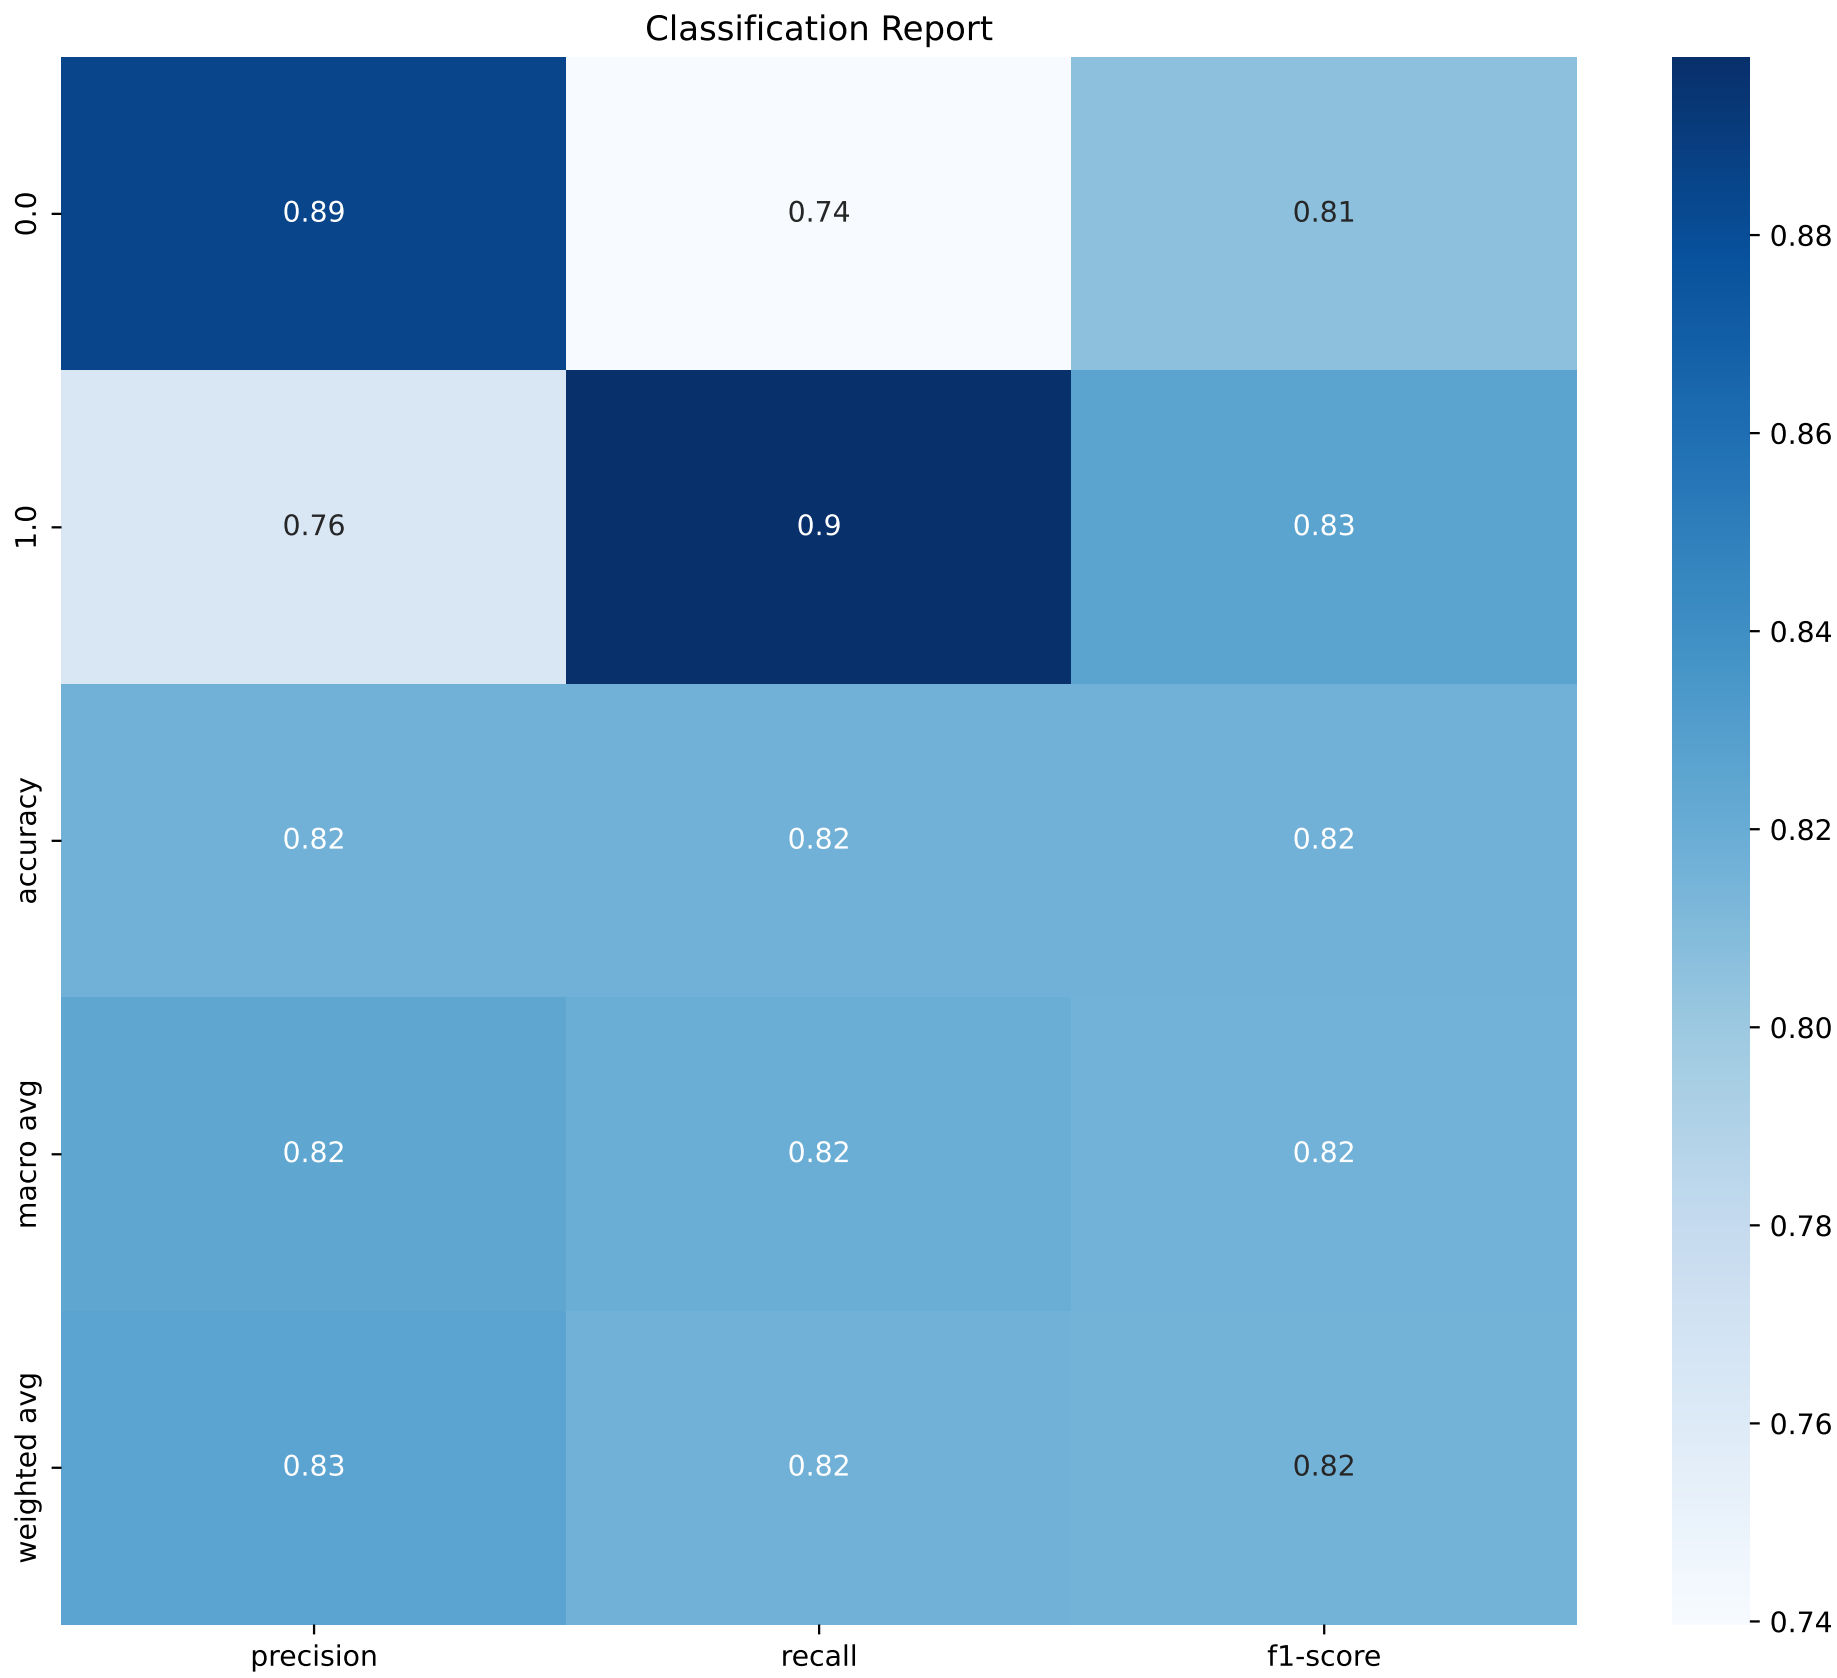
\includegraphics[width=0.5\textwidth]{C:/Users/marco/OneDrive/Documents/GitHub/mlops-netflix/mdr/plots/ClassificationReport.png}
				\caption{Classification Report}
				\label{fig:Classification_Report}
			\end{figure}
			\FloatBarrier
		\item \textbf{Confusion Matrix} (Figure 5): The confusion matrix provides a summary of the classification results by showing the true positive, true negative, false positive, and false negative values. In this project, the confusion matrix showed that the model was able to accurately classify a majority of the test cases, with relatively few misclassifications.
		\begin{figure}[H]
			\centering
			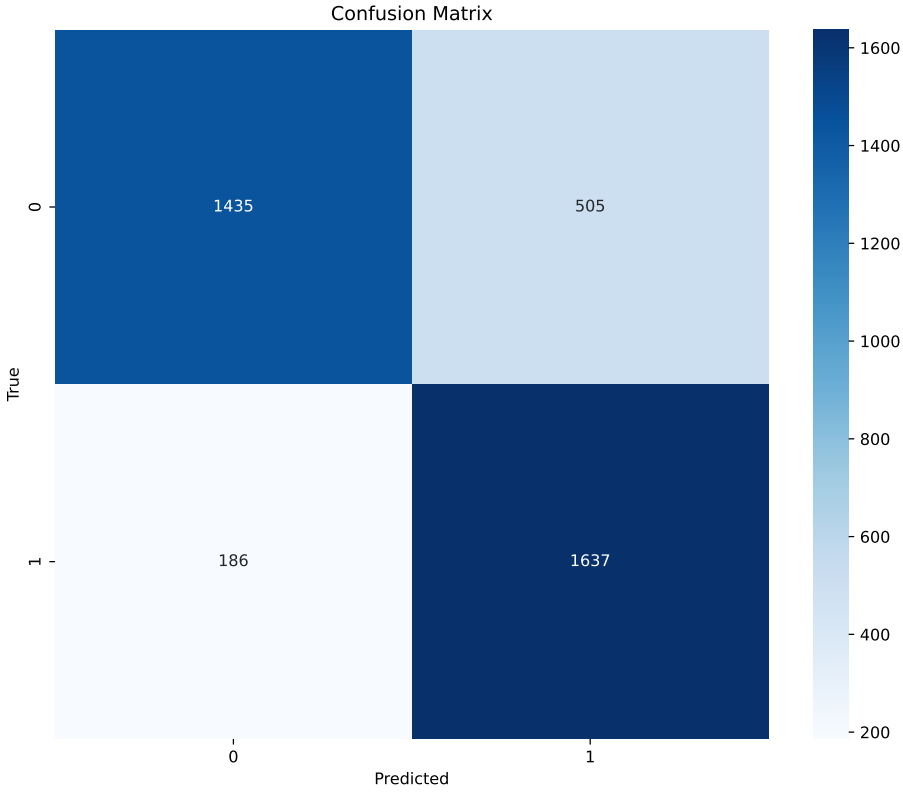
\includegraphics[width=0.5\textwidth]{C:/Users/marco/OneDrive/Documents/GitHub/mlops-netflix/mdr/plots/ConfusionMatrix.png}
			\caption{Confusion Matrix}
			\label{fig:Confusion_Matrix}
		\end{figure}
		\FloatBarrier
		\item \textbf{ROC Curve and AUC} (Figure 6): The Receiver Operating Characteristic (ROC) curve is a graphical representation of a classifier's ability to distinguish between classes. The Area Under the Curve (AUC) provides a single scalar value to measure the overall performance of the model. An AUC close to 1 indicates excellent model performance. The ROC curve generated in this project demonstrated that the Random Forest model had a high AUC, reflecting its strong ability to distinguish between different show profiles.
		\begin{figure}[H]
			\centering
			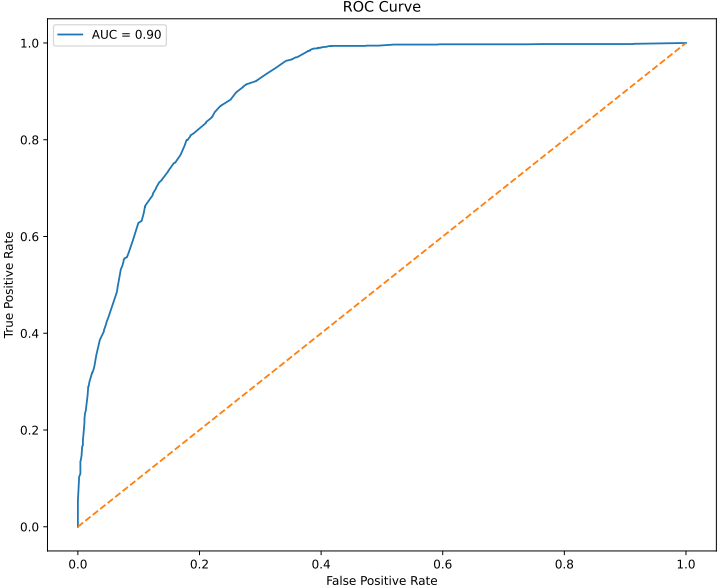
\includegraphics[width=0.5\textwidth]{C:/Users/marco/OneDrive/Documents/GitHub/mlops-netflix/mdr/plots/RocCurve.png}
			\caption{ROC Curve with AUC = 0.90}
			\label{fig:roc_curve}
		\end{figure}
		\FloatBarrier
		\item \textbf{Precision-Recall Curve} (Figure 7): The Precision-Recall curve is particularly useful when dealing with imbalanced datasets. It provides insight into the trade-offs between precision (the ability of the classifier not to label a negative sample as positive) and recall (the ability to find all positive samples). The curve for this project showed a good balance between precision and recall, indicating that the model effectively identifies relevant shows for recommendation.
		\begin{figure}[H]
			\centering
			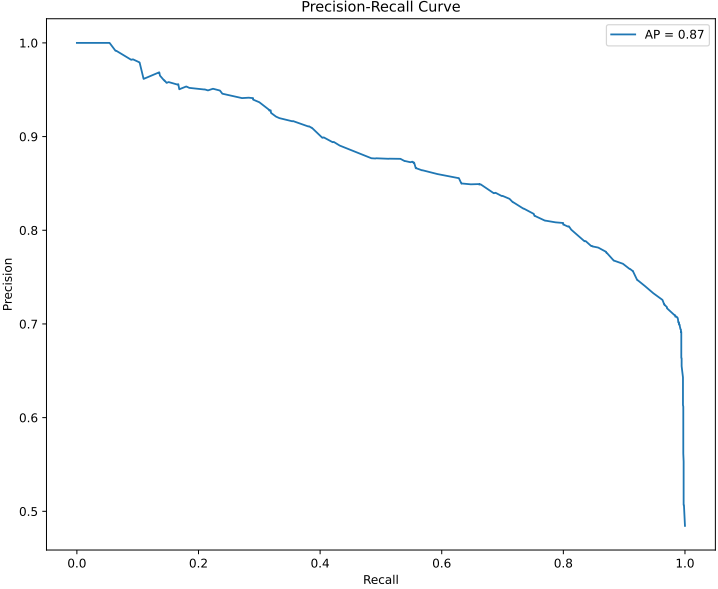
\includegraphics[width=0.5\textwidth]{C:/Users/marco/OneDrive/Documents/GitHub/mlops-netflix/mdr/plots/PrecisionRecallCurve.png}
			\caption{Precision-Recall Curve with AP = 0.87}
			\label{fig:precision_recall_curve}
		\end{figure}
		\FloatBarrier
		\item \textbf{Feature Importance} (Figure 8): An analysis of feature importance within the Random Forest model revealed which features contributed most to the prediction process. The most important features included certain genres, release years, and duration, which were consistently influential in determining the show's profile.
		\begin{figure}[H]
			\centering
			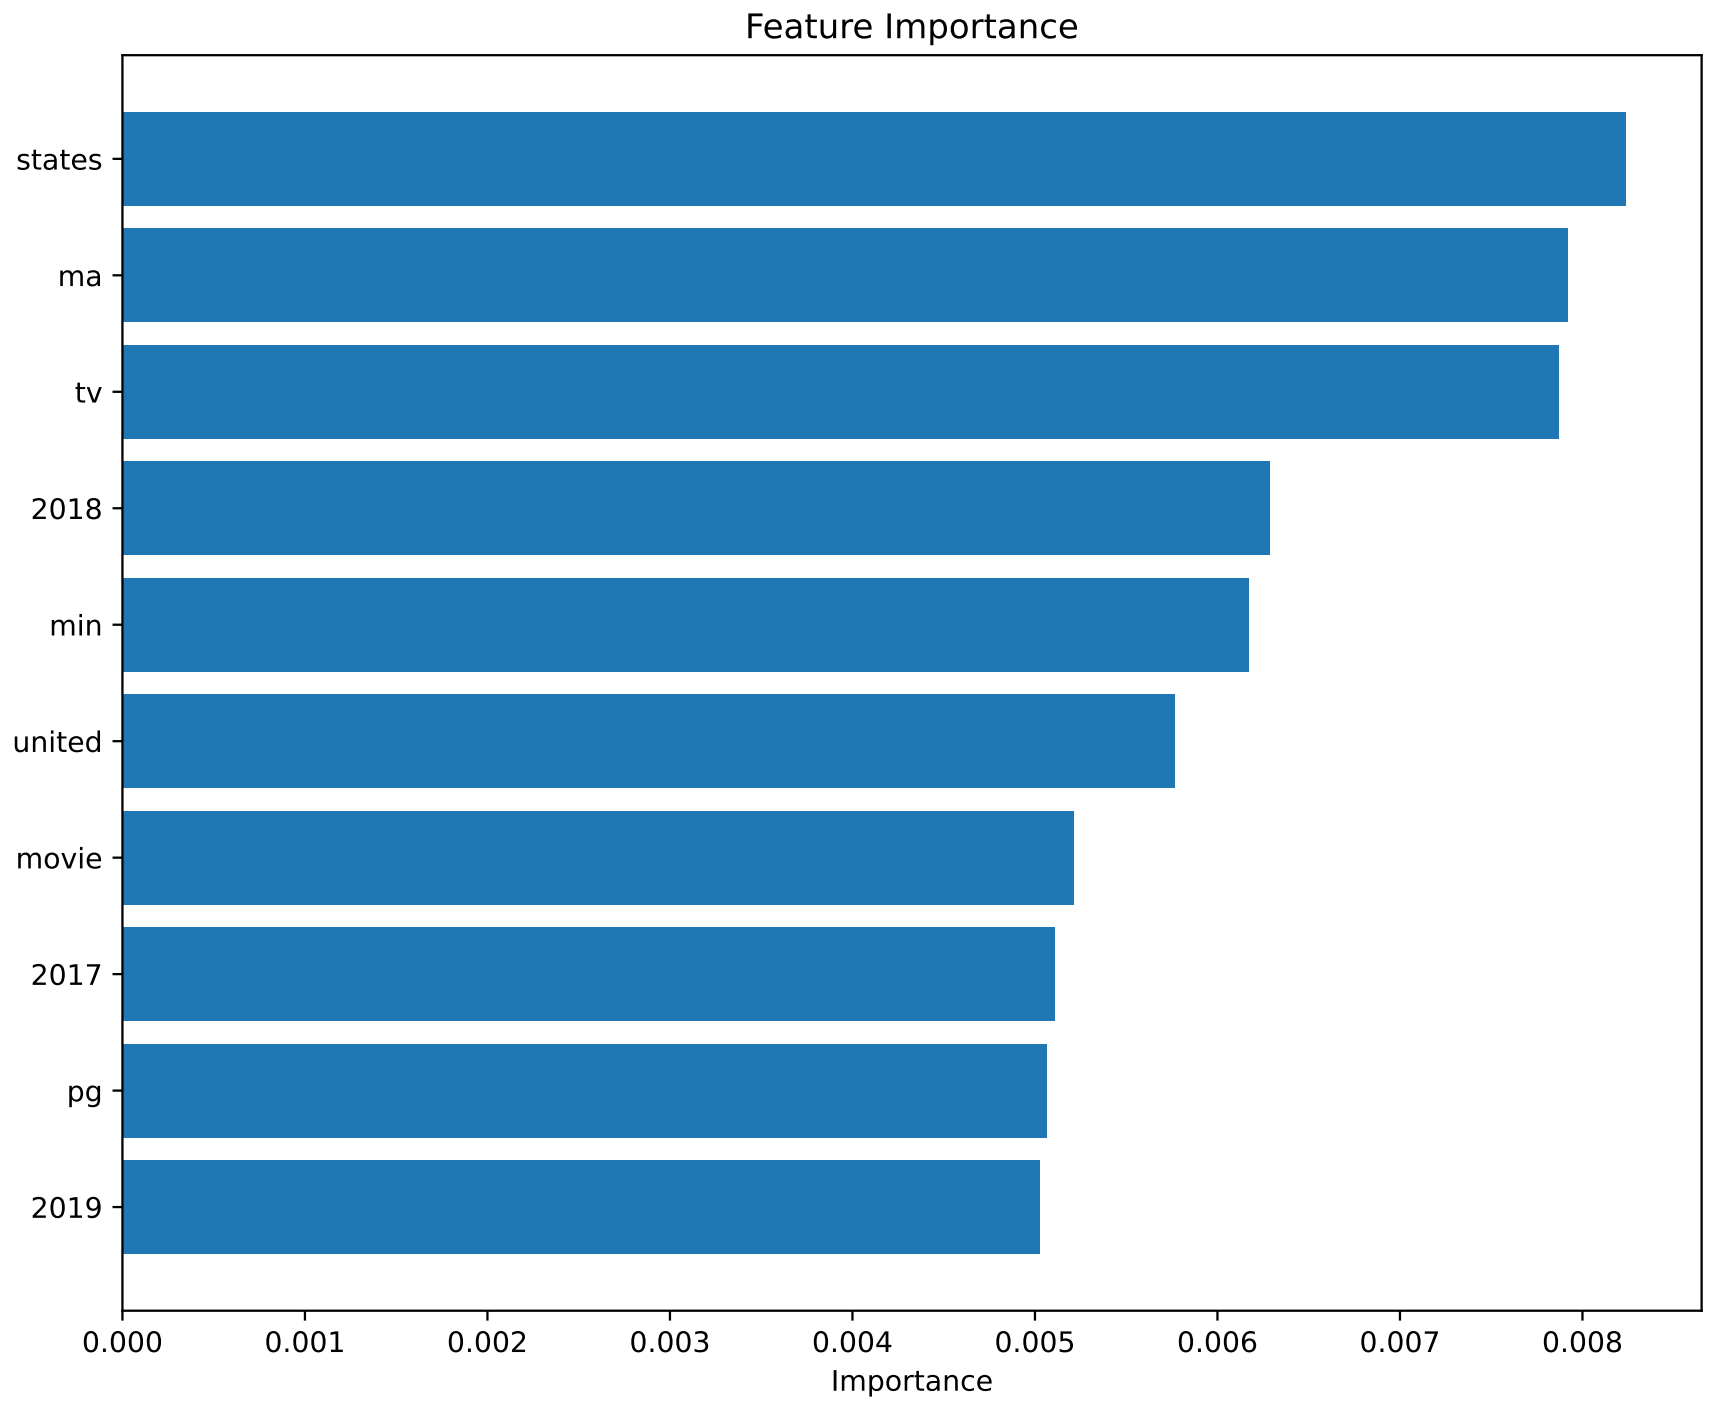
\includegraphics[width=0.5\textwidth]{C:/Users/marco/OneDrive/Documents/GitHub/mlops-netflix/mdr/plots/FeatureImportance.png}
			\caption{Feature Importance Analysis}
			\label{fig:feature_importance}
		\end{figure}
		\FloatBarrier
	\end{itemize}
	\section{Model Training and Testing}
	The dataset used in this project consists of 7130 records, with a significant class imbalance where the majority of the ratings are "Dislike" (5582 out of 7130). Given the size of the dataset and the class imbalance, specific measures were taken to ensure robust model training and evaluation.
	\subsection{Data Splitting and Balancing}
	The dataset was split into a training set and a test set, with 80\% of the data used for training and 20\% for testing. This division was chosen as it provides a sufficient amount of data for both training and testing, ensuring that the model can learn effectively while also being evaluated on a significant portion of the data.
	
	To address the issue of class imbalance, the Synthetic Minority Over-sampling Technique (SMOTE) was employed. SMOTE was applied to the training data to oversample the minority class ("Like" ratings), thereby creating a more balanced dataset. This approach helps prevent the model from being biased towards the majority class, which could otherwise lead to poor generalization.
	\subsection{Training Process}
	The training process involved the use of a Random Forest classifier with 100 estimators. The model was trained on the transformed feature set, which was created using the TF-IDF vectorization technique applied to the textual data. The Random Forest classifier was chosen for its ability to handle large datasets with numerous features and its robustness against overfitting.
	\subsection{Evaluation Metrics}
	The model's performance was evaluated using several metrics, including accuracy, precision, recall, F1-score, and the Area Under the Curve (AUC) for the ROC curve. Additionally, a Precision-Recall curve was generated to further assess the model's performance, particularly for the minority class ("Like" ratings). 
	
	Given the class imbalance, special attention was paid to the recall and F1-score metrics to ensure that the model was effectively identifying the minority class without being overwhelmed by the majority class. The application of SMOTE, combined with these evaluation metrics, provided a comprehensive understanding of the model's performance and its ability to generalize to unseen data.
	\section{Discussion \& Conclusion}
	The implementation of a Random Forest classifier within a K-Means clustering framework has proven to be an effective approach for developing a recommendation system for a streaming platform. The combination of these machine learning techniques allowed for the creation of distinct user profiles and accurate recommendations based on user preferences.
	The K-Means clustering algorithm was instrumental in segmenting the shows into distinct clusters, each representing a unique profile of user tastes. The silhouette score was employed to determine the optimal number of clusters, ensuring that the clustering was both meaningful and effective. The transformation of textual data into numerical features using the TF-IDF method enabled the model to process a wide range of variables, including titles, genres, and cast names, which were critical for accurately predicting user preferences.
	
	The Random Forest classifier further enhanced the system by providing robust classification and recommendation capabilities. Its ability to handle large datasets with numerous features, coupled with its resistance to overfitting, made it an ideal choice for this project. The evaluation metrics, including the confusion matrix, ROC curve, precision-recall curve, and feature importance analysis, all indicated that the model performed well, achieving an overall accuracy of 82\%.
	
	However, the system is not without its limitations. The recommendation system could potentially fall into a "filter bubble," where users are only recommended content similar to what they have already watched, thereby limiting exposure to a broader range of content. Future work could involve incorporating additional machine learning techniques, such as deep learning, to further refine the recommendations and address these limitations.
	
	In conclusion, this project demonstrates the effectiveness of combining K-Means clustering and Random Forest classification to develop a personalized recommendation system. The system successfully creates user profiles based on viewing habits and preferences, and provides accurate and relevant content recommendations, thereby enhancing the user experience on the streaming platform.
	\section{Future Work}
	While the current implementation of the recommendation system is robust, several avenues for future improvement exist:
	\begin{itemize}
		\item \textbf{Incorporation of Deep Learning}: Integrating deep learning models, such as neural networks, could enhance the system's ability to learn complex patterns in user behavior and preferences, potentially improving recommendation accuracy.
		\item \textbf{Exploration of Hybrid Models}: Combining collaborative filtering with content-based filtering and other hybrid approaches could further refine the recommendations by leveraging both user-item interactions and item content.
		\item \textbf{Ethical Considerations}: Addressing ethical concerns, such as user privacy and the potential for reinforcing biases in recommendations, will be crucial as the system evolves. Ensuring transparency and fairness in the recommendation process should be a priority.
	\end{itemize}
	The ongoing development and refinement of the recommendation system will aim to provide even more personalized and diverse content suggestions, ultimately leading to a richer and more satisfying user experience.
	\section*{Acknowledgments}
	The dataset used in this project was sourced from Kaggle, specifically the "Netflix Movies and TV Shows" dataset provided by Rahul Vyas. The dataset can be accessed at \url{https://www.kaggle.com/datasets/rahulvyasm/netflix-movies-and-tv-shows}.
	\bibliographystyle{ACM-Reference-Format}
	\begin{thebibliography}{00}
		\bibitem{kaggle_dataset} Rahul Vyas. Netflix Movies and TV Shows Dataset. Retrieved from \url{https://www.kaggle.com/datasets/rahulvyasm/netflix-movies-and-tv-shows}.
		\bibitem{netflix_ratings} Rishit Javia. Netflix Movie Rating Dataset. Retrieved from \url{https://www.kaggle.com/datasets/rishitjavia/netflix-movie-rating-dataset}.
	\end{thebibliography}
	
\end{document}
